1. Οι μεταβλητές στη C\# δηλώνονται χρησιμοποιώντας τον τύπο δεδομένων ακολουθούμενο από το όνομα της μεταβλητής. Μπορούν να αρχικοποιηθούν κατά την δήλωση ή αργότερα στον κώδικα. Τα ονόματα ξεκινούν με γράμμα ή με κάτω παύλα \_ . Οι υπόλοιποι χαρακτήρες μπορούν να είναι γράμματα, αριθμοί, ή \_ . Η γλώσσα είναι case-sensitive (number != Number). 

\begin{listing}[htbp]
\begin{minted}[]{csharp}
int number;
string message = "Hello, world!";
bool isTrue = true;
double Number = 3.14;
\end{minted}
\caption{Δηλώσεις μεταβλητών}
\label{flagExec}
\end{listing}

2. Οι συναρτήσεις στη C\# ονομάζονται μέθοδοι. Δηλώνονται με τον τύπο δεδομένων της επιστρεφόμενης τιμής (void εάν δεν επιστρέφουν τιμή), ακολουθούμενο από το όνομα της μεθόδου και τις παραμέτρους.

\begin{listing}[htbp]
\begin{minted}[]{csharp}
// Defining a simple function
void PrintMessage(string message)
{
    Console.WriteLine(message);
}

// Calling the function
PrintMessage("This is a function call");
\end{minted}
\caption{Απλή συνάρτηση}
\label{flagExec}
\end{listing}

3. Δομές επανάληψης (loops). Προσφέρονται διάφοροι τύποι επαναλήψεων, όπως 'for', 'while' και 'do-while'. Η σύνταξή τους είναι όπως στις C/C++.

\begin{listing}[htbp]
\begin{minted}[]{csharp}
for (int i = 0; i < 5; i++)
{
    Console.WriteLine("Number: " + i);
}
\end{minted}
\caption{Βρόχος που τυπώνει τους αριθμούς 0 έως και 4}
\label{flagExec}
\end{listing}

4. Οι εντολές if-else, χρησιμοποιούνται και αυτές με τον ίδιο τρόπο όπως στις C/C++.

\begin{listing}[htbp]
\begin{minted}[]{csharp}

int grade = 7;
if (grade >= 5)
{
    Console.WriteLine("PASS");
}
else
{
    Console.WriteLine("FALL");
}
\end{minted}
\caption{Απλό if - else statement}
\label{flagExec}
\end{listing}

5. Όλοι οι τύποι που μπορούν να οριστούν στην γλώσσα δίνονται συγκεντρωτικά στην εικόνα \ref{fig:types} \cite{typesbook}.

\begin{figure}[h!]
  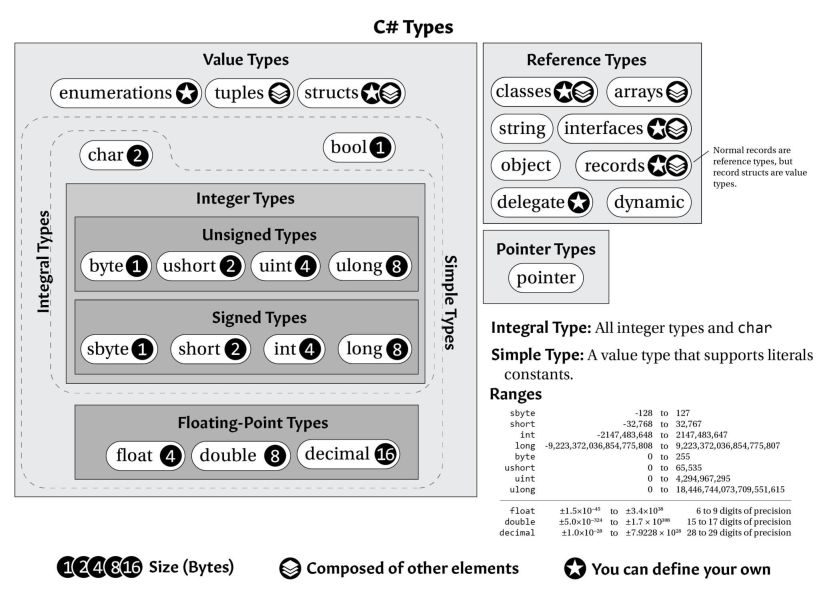
\includegraphics[width=\fullwidthimage]{images/csharptypes.jpg}
  \caption{Τύποι της C\#}
  \label{fig:types}
\end{figure}

